This part of the thesis focuses on the equivalence between \wlnn and \gnn. We will begin by providing a preliminary section that formalizes all the concepts used in the proof and introduces a general notation. Afterward, we will dedicate a separate section to present and prove three theorems. These theorems combined conclude the equivalence.

\section{Preliminaries}\label{sec:pre_lim}
This section will introduce and formalizes all concepts used throughout the proof and the rest of the thesis. We start with general notations, introduce a general graph definition, and familiarize the reader with the Weisfeiler-Leman algorithm. We will introduce each framework independently, first the \wlnn and then \gnn. In the end, we will briefly introduce important properties of collections of functions computed by both methods.

\subsection{General Notation}
Let $\Nb$ denote the set of natural numbers such that $\Nb := \{0, 1,2, \ldots \}$. By $[n]$, we denote the set $\{0, \ldots, n\} \subset \mathbb{N}$ for each $n \in \mathbb{N}$. Further, with $\MSopen \ldots \MSclose$, we denote a multiset formally defined as a 2-tuple $(X, m)$, where $X$ is a set of all unique elements and $m: X \rightarrow \mathbb{N}_{\geq 1}$ a mapping that maps each element in $X$ to the number of its occurrences in the multiset.

\subsection{Graphs}
We will briefly introduce a formal definition for graphs and coloring on graphs. Starting with the definition of a graph.

\begin{definition}[Graph]
A graph $G$ is defined as a 3-tuple denoted by $G \coloneqq (V, E, l)$. This tuple consists of a set of nodes $V \subset \Nb$, a set of edges $E \subseteq V \times V$, and a labeling function $l: M \rightarrow \Sigma$. The domain $M$ of the labeling function can be either $V$, $V \cup E$, or $E$, and the codomain $\Sigma$ is an alphabet with $\Sigma \subseteq \mathbb{N}^k$, where $k \in \Nb$ is arbitrary.
In the context of this thesis, the assigned values by the labeling function are referred to as either labels or features, depending on the dimension of $\Sigma$. In detail, if $k=1$, we usually refer to the values as labels, otherwise as features. Additionally, the set of all graphs is denoted by $\cG$.

Furthermore, a graph $G$ can be either directed or undirected based on the definition of its set of edges $E$. If $E \subseteq \{(v,u) \mid v,u \in V\}$, it represents a directed graph, whereas if $E \subseteq \{(v, u) \mid v,u \in V, v\neq u\}$ such that for every $(v,u) \in E$ there exists $(u,v) \in E$, it defines an undirected graph. Additionally, for ease of notation, we will use $V(G)$ and $E(G)$ to denote the set of nodes and the set of edges of $G$, respectively, as well as $l_G$ to denote the label function of $G$. Further, with $\mathcal{N}(v)$ for $v \in V(G)$ we denote the set of neighbors of $v$ defined as $\mathcal{N}(v) \coloneqq \{u \mid (u, v) \in E(G)\}$, and with $d(v)$ for $v \in V(G)$ the degree of node $v$, defined as $d(v) := |\mathcal{N}(v)|$.
\end{definition}

We continue with the definition of a graph coloring.

\begin{definition}[Graph Coloring]
A coloring of a Graph $G$ is a function $C: V(G) \rightarrow \mathbb{N}$ that assigns each node in the graph a color (here, a positive integer). Further, a coloring $C$ induces a partition $\cP$ on the set of nodes, for which we define $C^{-1}$ being the function that maps each color $c \in \mathbb{N}$ to its class of nodes with $C^{-1}(c) = \{ v\in V(G) \mid C(v) = c\}$. In addition, we define $\hist_{G, C}$ as the histogram of graph $G$ with coloring $C$ that maps every color in the image of $C$ under $V(G)$ to the number of occurrences. In detail, $\forall c \in \mathbb{N}: \hist_{G, C}(c) \coloneqq | \{ v \in V(G) \mid C(v) = c \} | = | C^{-1}(c) |$.
\end{definition}

\subsubsection{Permutation-invariance and -equivariance}
We use $S_n$ to denote the symmetric group over the elements $[n]$ for any $n \in \Nb$. $S_n$ consists of all permutations over these elements. Let $G$ be a graph with $V(G) = [n]$, applying a permutation $\pi \in S_n$ on $G$, is defined as $G_\pi \coloneqq \pi \cdot G$ where $V(G_\pi) = \{\pi(0), \ldots, \pi(n) \}$ and $E(G_\pi) = \{ (\pi(v), \pi(u)) \mid (v,u) \in E(G)\}$. We will now introduce two key concepts for classifying functions on graphs.

\begin{definition}[Permutation Invariant]
    Let $f: \mathcal{G} \rightarrow \mathcal{Y}$ be an arbitrary function, then $f$ is \textit{permutation-invariant} if and only if for all $G \in \mathcal{G}$, where $n_G \coloneqq |V(G)|$ and for every $\pi \in S_{n_G}$: $f(G) = f(\pi \cdot G)$.
\end{definition}

\begin{definition}[Permuation Equivariant]
    Let $f: \mathcal{G} \rightarrow \mathcal{Y}$ be an arbitrary function, then $f$ is \textit{permuation-equivariant} if and only if for all $G \in \mathcal{G}$, where $n_G \coloneqq |V(G)|$ and for every $\pi \in S_{n_G}$: $f(G) = \pi^{-1} \cdot f(\pi \cdot G)$.
\end{definition}

\subsection{Weisfeiler and Leman Algorithm}\label{sec:1-WL Definition}
The Weisfeiler-Leman algorithm consists of two main parts: the coloring algorithm and the graph isomorphism test. We will introduce each part individually and present some implications afterward.

\subsubsection{The Weisfeiler-Leman Graph Coloring Algorithm}
The $\wl$ algorithm computes a node coloring of its input graph in each iteration. In detail, a color is assigned to each node based on the colors of its neighbors and its own current color. The algorithm continues until convergence is reached, resulting in the final coloring of the graph. We will now formally define this procedure and provide an illustrative example in \cref{fig:1wl_example}.

\begin{definition}[$\wl$ Algorithm]
    Let $G = (V, E, l)$ be a labeled graph. In each iteration $i$, the \wl algorithm computes a node coloring $C_i: V(G) \rightarrow \mathbb{N}$. In the initial iteration $i=0$, the coloring is set to $C_0 = l$ if $l$ exists. Otherwise, for all $v \in V(G): C_0(v) = c$ with $c \in \Nb$ being an arbitrary but fixed constant. For $i > 0$, the algorithm assigns a color to $v \in V(G)$ as follows:
    \begin{equation*}
        C_i (v) = \textsf{RELABEL}(C_{i-1}(v),  \ \MSopen C_{i-1}(u) \mid u \in \mathcal{N}(v) \MSclose),
    \end{equation*}
    where $\textsf{RELABEL}$ injectively maps the above pair to a unique, previously not used, color. The algorithm terminates when the number of colors between two iterations does not change, meaning the algorithm terminates after iteration $i$ if the following condition is satisfied:
    \begin{equation*}
        \forall v,w \in V(G):  C_i(v) = C_i(w) \iff C_{i+1}(v) = C_{i+1}(w).
    \end{equation*}
    Upon terminating we define $C_{\infty} \coloneqq C_i$ as the stable coloring, such that $\wl(G) \coloneqq C_\infty$.
\end{definition}

The colorings computed in each iteration always converge to the final one, such that the algorithm always terminates. In more detail, \cite{Gro2017} showed that it always holds after at most $|V(G)|$ iterations. For an illustration of this algorithm, see \cref{fig:1wl_example}. Moreover, based on the work of \cite{Pai+87} about efficient refinement strategies, \cite{Car+82} proved that the stable coloring $C_\infty$ can be computed in time $\mathcal{O}(| V(G) | + |E(G)| \cdot \log | V(G) |)$.

\begin{figure}[H]
    \centering
    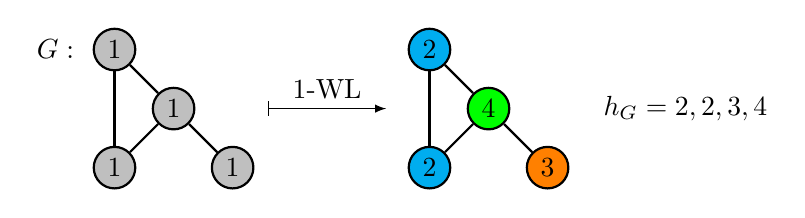
\begin{tikzpicture}
    \tikzset{line/.style={draw,thick}}
    \tikzset{arrow/.style={line,->,>=stealth}}
    \tikzset{node/.style={circle,inner sep=0pt,minimum width=15pt}}
    
    \draw (-1.5,0.75) node {$G:$};
    \node[line,node,fill=lightgray] (x1) at (-0.75, 0.75) {1};
    \node[line,node,fill=lightgray] (x2) at (-0.75, -0.75) {1};
    \node[line,node,fill=lightgray] (x3) at (0.75, -0.75) {1};
    \node[line,node,fill=lightgray] (x4) at (0, 0) {1};
    
    \path[line] (x1) to (x2);
    \path[line] (x1) to (x4);
    \path[line] (x2) to (x4);
    \path[line] (x3) to (x4);

    \draw [|-latex] (1.2,0) -- node [text width=2.5cm,midway,above,align=center ] {1-WL} (2.7,0);
    

    \node[line,node,fill=cyan] (x1) at (-0.75 + 4.0, 0.75) {2};
    \node[line,node,fill=cyan] (x2) at (-0.75 + 4.0, -0.75) {2};
    \node[line,node,fill=orange] (x3) at (0.75 + 4.0, -0.75) {3};
    \node[line,node,fill=green] (x4) at (0 + 4.0, 0) {4};
    
    \path[line] (x1) to (x2);
    \path[line] (x1) to (x4);
    \path[line] (x2) to (x4);
    \path[line] (x3) to (x4);

    \draw (6.5, 0.0) node {$h_G = \MSopen 2, 2, 3, 4 \MSclose$};

    
    
    \end{tikzpicture}

    \caption{An example of the final coloring computed by applying the \wl algorithm on the graph $G$. The graph $G$ consists of $4$ nodes with all their labels being set to the same color.}
    \label{fig:1wl_example}
\end{figure}

It is important to understand that since the algorithm was originally developed as a simple heuristic for the \textit{graph isomorphism problem}, which is an inherently discrete problem, the \wl algorithm in its simplest form, as we presented it here, does only work on graphs with discrete, one-dimensional node labels. Although it is quite easy to adapt the algorithm to respect discrete edge labels of a graph by using them as weights in the neighborhood aggregation (\cite{Shervashidze2011}), modifying its definition to work with continuous graph features is more complex. Numerous proposed modifications have been put forward to address this integration in the literature, such as those discussed by \cite{Mor+2016}. However, note that this particular topic will not be further investigated in this thesis, although its mention holds value for \cref{part2}.

\subsubsection{The Weisfeiler-Leman Graph Isomorphism Test}
The isomorphism test uses the \wl coloring algorithm and is defined as follows.

\begin{definition}[$\wl$ Isomorphism Test]
    To determine if two graphs $G, H \in \mathcal{G}$ are non-isomorphic ($G \ncong H)$, one applies the \wl coloring algorithm on both graphs ``in parallel'' and checks after each iteration if the occurrences of each color are equal, else the algorithm would terminate and conclude non-isomorphic. Formally, the algorithm concludes non-isomorphic in iteration $i$ if there exists a color $c$ such that: 
    \begin{equation*}
        |\{ v \in V(G) \mid C_i(v) = c\} | \neq |\{ w \in V(H) \mid C_i(w) = c\} |.
    \end{equation*}
\end{definition}

Note that this test is only sound and not complete for the \textit{graph isomorphism problem}. Counterexamples can be easily constructed where the algorithm fails to distinguish non-isomorphic graphs. See \cref{1-WL Counter Example} for a straightforward example of where this test fails that was discovered and proven by \cite{Cai1992}.
\begin{figure}[H]
    \centering
    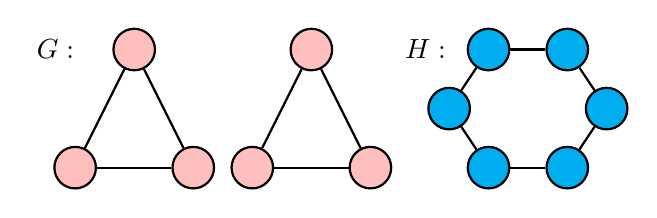
\begin{tikzpicture}

\tikzset{line/.style={draw,thick}}
\tikzset{arrow/.style={line,->,>=stealth}}
\tikzset{node/.style={circle,inner sep=0pt,minimum width=15pt}}

\draw (-1.0,0.75) node {$G:$};
\node[line,node,fill=pink] (x1) at (0, 0.75) {};
\node[line,node,fill=pink] (x2) at (-0.75, -0.75) {};
\node[line,node,fill=pink] (x3) at (0.75, -0.75) {};

\path[line] (x1) to (x2);
\path[line] (x1) to (x3);
\path[line] (x2) to (x3);

\node[line,node,fill=pink] (x1) at (2.25, 0.75) {};
\node[line,node,fill=pink] (x2) at (1.5, -0.75) {};
\node[line,node,fill=pink] (x3) at (3.0, -0.75) {};

\path[line] (x1) to (x2);
\path[line] (x1) to (x3);
\path[line] (x2) to (x3);

\draw (3.7, 0.75) node {$H:$};
\node[line,node,fill=cyan] (x1) at (3.75 + 0.25, 0) {};
\node[line,node,fill=cyan] (x2) at (4.25 + 0.25, 0.75) {};
\node[line,node,fill=cyan] (x3) at (5.25 + 0.25, 0.75) {};
\node[line,node,fill=cyan] (x4) at (5.75 + 0.25, 0) {};
\node[line,node,fill=cyan] (x5) at (5.25 + 0.25, -0.75) {};
\node[line,node,fill=cyan] (x6) at (4.25 + 0.25, -0.75) {};

\path[line] (x1) to (x2);
\path[line] (x2) to (x3);
\path[line] (x3) to (x4);
\path[line] (x4) to (x5);
\path[line] (x5) to (x6);
\path[line] (x6) to (x1);

\end{tikzpicture}
    \caption{This is an example of two graphs $G$ and $H$ that are non-isomorphic but cannot be distinguished by the \wl isomorphism test.}
    \label{1-WL Counter Example}
\end{figure}

\subsubsection{Implications of the \wl Algorithm}
One implication of the \wl algorithm and its isomorphism test is that, due to it not being complete for solving the \textit{graph isomorphism problem}, it gives rise to a related but weaker relation than the isomorphism relation ($\simeq$). We define this relation as follows.

\begin{definition}[\wl Relation]
    Let $\cX \subseteq \cG$. For any graphs $G,H \in \cX$ we will denote $G \wliso H$ if the \wl isomorphism test can not distinguish both graphs. Note that due to the soundness of this algorithm, if $G \not\wliso H$, we always can conclude that $G \not\simeq H$.
\end{definition}

The $\wliso$ relation can further be classified as an equivalence relation, as it is reflexive, symmetric and transitive. With this, we introduce a notation of its equivalence classes. Let $\cX \subseteq \cG$ and $G \in \cX$, then we denote with $\cX/\!{\wliso}(G): = \{ G' \in \cX \mid G \wliso G' \}$ its equivalence class.

Similarly, we define the notion \wldisc for collections of permutation invariant functions.

\begin{definition}[\wldisc]
    Let $\cX \subseteq \cG$. Further, let $\cC$ be a collection of permutation invariant functions from $\cX$ to $\Rb$. We say $\cC$ is \wldisc if for all graphs $G_1, G_2 \in \cX$ for which the \wl isomorphism test concludes non-isomorphic ($G_1 \not\wliso G_2$), there exists a function $h_{G_1, G_2} \in \cC$ such that $h_{G_1, G_2}(G_1) \neq h_{G_1, G_2}(G_2)$.
\end{definition}

\subsection{\wlnn}\label{sec:definition_wlnn}
As the \cref{sec:related_work_wl} shows, the $\wl$ algorithm is quite powerful in identifying a graph's substructures and distinguishing non-isomorphic graph pairs. With the \wlnn framework, we define functions that utilize this structural information to derive application-specific insights.

\begin{definition}[\wlnn]
    A \wlnn model consists of three components that are applied sequentially to its input: 1. the $\wl$ algorithm, 2. an encoding function $f_\text{enc}$ operating on graph colorings, and 3. an arbitrary multilayer perceptron $\mlp$. In detail, a \wlnn model computes the function $\cB$, that is defined as follows:
    \begin{align*}
        \cB: \cG \rightarrow \Rb^k, \ G \mapsto \mlp \circ f_{\text{enc}}(\MSopen \wl(G)(v) \mid v \in V(G) \MSclose),
    \end{align*}
    where $\wl(G)$ is the coloring computed by the $\wl$ algorithm when applied on $G$, and $k \in \Nb_{\geq 1}$ is a freely selectable hyperparameter. For a better understanding and an illustrative explanation, see \cref{fig:wlnn}.
\end{definition}

\begin{figure}[!htb]
    \centering
    \begin{tikzpicture}
    \definecolor{pastell_blue}{RGB}{133,154,202}
    \definecolor{pastell_green}{RGB}{192,223,211}
    \definecolor{pastell_pink}{RGB}{228,197,212}
    \tikzset{line/.style={draw,thick}}
    \tikzset{arrow/.style={line,->,>=stealth}}
    \tikzset{node/.style={circle,inner sep=0pt,minimum width=15pt}}
    
    \node[line,node,fill=gray] (x1) at (-0.75 - 0.8, 0.75) {};
    \node[line,node,fill=gray] (x2) at (-0.75 - 0.8, -0.75) {};
    \node[line,node,fill=gray] (x3) at (0.75 - 0.8, -0.75) {};
    \node[line,node,fill=gray] (x4) at (0 - 0.8, 0) {};
    
    \path[line] (x1) to (x2);
    \path[line] (x1) to (x4);
    \path[line] (x2) to (x4);
    \path[line] (x3) to (x4);

    \draw[arrow, thick] (0.1, 0.0) to (0.9, 0.0);

    \draw (2.15, 0.9) node {$\wlnn$:};
    \filldraw[draw=black, fill=gray!40, thick, rounded corners] (1.1, -0.7) rectangle (8.9, 0.7);

    \filldraw[draw=black, fill=green, thick, rounded corners] (1.2, -0.6) rectangle (2.4, 0.6) node[midway,align=center]{$\wl$};

    \draw[arrow, thick] (2.5, 0.0) to (2.9, 0.0);
    
    \draw (3.5, 0.0) node {$\MSopen \ldots \MSclose$};

    \draw[arrow, thick] (4.1, 0.0) to (4.5, 0.0);

    \filldraw[draw=black, fill=cyan, thick, rounded corners] (4.6, -0.6) rectangle (5.8, 0.6) node[midway,align=center]{$f_{\text{enc}}$};

    \draw[arrow, thick] (5.9, 0.0) to (6.3, 0.0);
    \draw (6.7, 0.0) node {$\begin{pmatrix*} \vdots \end{pmatrix*}$};
    \draw[arrow, thick] (7.1, 0.0) to (7.5, 0.0);

    \filldraw[draw=black, fill=pink, thick, rounded corners] (7.6, -0.6) rectangle (8.8, 0.6) node[midway,align=center]{$\mlp$};

    \draw[arrow, thick] (9.1, 0.0) to (9.9, 0.0);
    \draw (10.3, 0.0) node {$42$};
    
\end{tikzpicture}

    \caption{This simplified illustration explains the components that make up a \wlnn model and how each one processes the input further. In detail, the model takes the graph on the left as input and first applies the \wl algorithm, thereby obtaining a multiset of the colors assigned by the algorithm. Then the encoding function $f_\text{enc}$ is applied, resulting in a fixed-sized vector that is further processed by the multilayer perceptron $\mlp$. The output of the $\mlp$ is then propagated as the \wlnn models output, here the number $42$.}
    \label{fig:wlnn}
\end{figure}

It is worth noting that this definition can be easily adjusted to accommodate node- or edge-level tasks by applying the encoding function $f_\text{enc}$ and the multilayer perceptron $\mlp$ elementwise to the colors of the multiset. However, for the purposes of this thesis, we will not delve into these variations, as our main focus will be on graph-level tasks such as graph classification or regression, which possess greater theoretical interest and are more prevalent in most datasets. Furthermore, all the theoretical findings presented in this thesis can be straightforwardly adapted to \wlnn models designed for node- or edge-level tasks.

\subsection{Graph Neural Networks (Message-Passing)}\label{sec:GNN Defintion}
A \textsf{Graph Neural Network} (\gnn) is a composition of multiple layers, where each layer computes a new feature for each node and edge. Each \gnn layer thus technically obtains a new graph structurally identical to the previous one but with new feature information. After an input graph has been passed through all layers, a final readout function is applied that pools all graph features and derives a task-related output. With this, it is possible to apply a \gnn to every graph, regardless of its size, as the ``computation'' will only take place on the nodes and edges of the graph.

Note that in the following, we will restrict the definition only to consider node features; however, one can easily extend it to include edge features as well.

\begin{definition}[\textsf{Graph Neural Network}]\label{def:gnn}
    Let $G = (V, E, l)$ be an arbitrary graph. A \gnn is a composition of multiple layers and a final readout function where each layer $t$ is represented by a function $f^{(t)}$. The initial layer at $t=0$ is a function of the format $f^{(0)}: V(G) \rightarrow \mathbb{R}^{1 \times d}$ that is consistent with $l$ and translates all labels into a vector representation. In contrast, for every $t > 0$, $f^{(t)}$ is recursively defined as:
    \begin{align*}
        f^{(t)}(v) = f^{(t)}_{\text{merge}} (f^{(t-1)}(v), \  f^{(t)}_{\text{agg}}( \MSopen f^{(t-1)}(w) \mid w \in \mathcal{N}(v) \MSclose )),
    \end{align*}
    where $f^{(t)}_{\text{merge}}$ is an arbitrary function that maps the aforementioned tuple to a vector, effectively ``merging'' them, while $f^{(t)}_{\text{agg}}$ is an arbitrary function that maps the multiset to a vector, effectively ``aggregating'' it.
    
    The readout function, referred to as $\textsf{Readout}$, is applied after the input graph has been passed subsequently through all layers and is defined as follows:
    \begin{align*}
        \textsf{Readout}(\MSopen f^{(t)}(v) \mid v \in V(G) \MSclose).
    \end{align*}
    This function pools the information from every node feature, processes it, and calculates a fixed-sized output vector for the entire graph.
    
    In summary, a \gnn model will compute the function $\cA$ defined as follows:
    \begin{align*}
        \cA: \cG \rightarrow \Rb^k, \ G \mapsto \textsf{Readout}(\MSopen f^{(T)}(v) \mid v \in V(G) \MSclose),
    \end{align*}
    where $T$ is the number of layer of the \gnn, and $k \in \Nb$ an arbitrary constant. To enable end-to-end training of a \gnn, it is essential that all its components are differentiable. Therefore, we require all $f^{(t)}_{\text{merge}}$ and $f^{(t)}_{\text{agg}}$ functions for all $t \in [T]$, along with the final $\textsf{Readout}$ function, to be differentiable.
\end{definition}
Note that, due to our definition of the ``aggregation'' and the ``readout'' function to operate over multisets, both functions are permutation invariant by definition. With this, we can conclude that the total composition $\cA$ is permutation invariant, and with similar reasoning, it is also differentiable. This property enables us to train $\cA$ like any other machine learning method in an end-to-end fashion, regardless of the underlying encoding used for graphs. 

Furthermore, \gnns following this definition are regarded as \textsf{Message-Passing-Neural-Network (MPNN)}. This designation stems from each node exchanging information with its direct neighbors in each layer. As a result, information during the processing of a graph is propagated by passing many messages across the graph; thus, these layers are also referred to as \textit{message-passing} layers. As outlined in the introduction to this thesis, we will solely focus on \gnns utilizing the \textit{message-passing} architecture. Therefore we will use the term \gnn and \textsf{MPNN} interchangeably throughout this thesis. The definition and notation used here are inspired by \cite{Morris2018} and \cite{Xu2018}.

To bridge the gap from the theoretical definition to practical instances of the definition, we will now introduce three distinct \gnn architectures. Specifically, we will explore the \textsf{Graph Attention Network} (\gat) developed by \cite{Velivckovic2017}, \textsf{Graph Convolutional Network} (\gcn) proposed by \cite{Kip+2017}, and the \textsf{Graph Isomorphism Network} (\gin) introduced by \cite{Xu2018}. These architectures will serve as empirical baselines in \cref{part2}. Additionally, we will also elaborate on the reasons for this choice of models in \cref{part2} in \cref{sec:gnn_model_choice}. We listed the definitions of the \textit{message-passing} layers of each model in \cref{tab:models}.

\begin{table}[H]
    \centering
    \caption{Overview of the construction of the \textit{message-passing} layers and their respective learnable parameters by popular \gnn architectures. A complete definition of the \gat architecture including the attention coefficient $\alpha_{vu}$ can be found in \cref{def:gat} in the Appendix.}
    \resizebox{.975\textwidth}{!}{ 	\renewcommand{\arraystretch}{2.2}
    \begin{tabular}{c|c|c|c}
        \textbf{Model} & \textbf{Merge Function} & \textbf{Aggregation Function} & \textbf{Learnable Parameters}\\
        \hline
        \gat & $f^{(t)}_{\text{merge}} = \sigma (\alpha_{vv} \cdot f^{(t)}(v) + f^{(t)}_{\text{agg}} )$ & $f^{(t)}_{\text{agg}} = \nnsum_{u \in \cN(v)} \alpha_{vu} \cdot W^{(t)} \cdot f^{(t-1)}(u)$ & $\alpha_{vu}, W^{(t)}$ \\
        \hline
        \gcn & $f^{(t)}_{\text{merge}} = \text{ReLU}\biggl( \frac{W^{(t)}}{1 + d(v)} f^{(t-1)}(v) + f^{(t)}_{\text{agg}} \biggr)$ & $f^{(t)}_{\text{agg}} = \nnsum_{u \in \cN(v)} \frac{W^{(t)}}{\sqrt{(1 + d(v))\cdot (1 + d(u))}} f^{(t-1)}(u)$ & $W^{(t)}$
        \\
        \hline
        \gin & $f^{(t)}_{\text{merge}} = \mlp^{(t)} \biggl( \bigl( 1 + \epsilon^{(t)} \bigr) \cdot f^{(t-1)}(v) + f^{(t)}_{\text{agg}} \biggr)$ & $f^{(t)}_{\text{agg}} = \nnsum_{u \in \cN(v)} f^{(t-1)}(u)$ & $\epsilon^{(t)}, \mlp^{(t)}$
        \\
    \end{tabular}
    }
\end{table}\todo{Rally small technical detail, but i dont thinnk the attention value fits into my defintion of \gnns}

Commonly employed \textsf{Readout} functions in this context often involve straightforward pooling techniques like elementwise summation, mean calculation, or maximum extraction. These pooling operations are typically followed by a multilayer perceptron, which performs additional processing on the aggregated information. Although more sophisticated pooling operations exist, such as \textsc{Set2Set} developed by \cite{Vinyals2015}, \cite{Xu2018} showed that given the correct configuration, the elementwise summation pooling function combined with a following multilayer perceptron suffices to create a \gnn that is as expressive as the \wl algorithm in distinguishing non-isomorphism.

\section{Theoretical Connection}\label{sec:theo_connections}
This section forms the core of our theoretical investigation, where we explore the equivalence between two frameworks: \wlnn and \gnn. We present two theorems to establish this equivalence, each showing a separate equivalence direction. By combining these theorems, we conclusively establish the equivalence. To maintain clarity and rigor, we will prove each theorem separately afterward in a corresponding subsection.

In particular, the theorem will establish a theoretical connection between the frameworks when applied to a finite collection of graphs, which we denote by $\cX$ with $\cX \subset \cG$.

\begin{theorem}[Finite Case: ``$\text{GNN} \subseteq \wlnn$'']\label{theorem:gnn_in_1wl}
    Let $\cC$ be a collection of functions from $\cX$ to $\Rb$ computable by \gnns, then $\cC$ is also computable by \wlnn.
\end{theorem}

\begin{theorem}[Finite Case: ``$\wlnn \subseteq \text{GNN}$'']\label{theorem:1wl_in_gnn}
    Let $\cC$ be a collection of functions from $\cX$ to $\Rb$ computable by \wlnn, then $\cC$ is also computable by \gnns.
\end{theorem}

With these two theorems, the equivalence between both frameworks follows. Specifically, every function computed by \wlnn working over any arbitrary but finite $\cX \subset \cG$ is also computable by a \gnn, and vice versa. Consequently, we can draw the following corollary:
\begin{corollary}
    For an arbitrary function $f$ working over $\cX$ to $\Rb$: The function $f$ is computable by a \wlnn model, if and only if, the function $f$ is computable by a \gnn model.
\end{corollary}
As we move towards the empirical evaluation in \cref{part2}, it is evident that if we test a \wlnn model on any of the benchmark datasets, it can theoretically achieve the same level of performance as a \gnn model. Notice that we did not leverage any constraints on the encoding of graphs throughout the two theorems and their corresponding proves but instead kept it general.


\subsection{Proof of \cref*{theorem:gnn_in_1wl}: ``$\gnn \subseteq \wlnn$''}\label{sec:proof_theorem:1wl_in_gnn}
We will prove \cref{theorem:1wl_in_gnn} by first introducing a set of lemmas, which will be leveraged in the proof of the theorem at the end of this section. The lemmas \cref{lem:encoding-indicator-func1,lem:encoding-indicator-func2}, and the proof of \cref{theorem:gnn_in_1wl} extend the results by \cite{Chen2019}.

To begin, we prove an essential insight that for any pair of graphs indistinguishable by the \wl isomorphism test, the output of any \wlnn model applied to both graphs is identical.
\begin{lemma}[\wlnn Equivalence]\label{lem:wl_relation_equivalence}
    Let $\cB$ be a function over $\cX$ computable by \wlnn, then for every pair of graphs $G_1, G_2 \in \cX:$ if $G_1 \wliso G_2$ then $\cB(G_1) = \cB(G_2)$.
\end{lemma}
\begin{proof}
    Assume the above. Let $\cB$ be an arbitrary function over $\cX$ computable by \wlnn, then $\cB$ is composed as follows: $\cB(\cdot) = \mlp \circ f_{\text{enc}} \MSopen \wl(\cdot)(v) \mid v \in V(\cdot) \MSclose$. Further, let $G_1, G_2 \in \cX$ be arbitrary graphs with $G_1 \wliso G_2$, then by definition of the $\wliso$ relation we know that $\wl(G_1) = \wl(G_2)$. With this, the equivalence follows, since this implies the equivalence of the multiset of colors for both graphs.
\end{proof}

As a consequence of this lemma, we establish that every function computable by \wlnn is also permutation invariant.
\begin{corollary}[\wlnn Permuation Invariance]\label{lem:wlnn_permutation_invariance}
    Let $\cB$ be a function over $\cX$ computable by \wlnn, then $\cB$ is permutation invariant.
\end{corollary}

\begin{proof}
    Assume the above. Let $G \in \cX$ be an arbitrary graph and $\pi$ a permutation of $V(G)$ the set of nodes, then we know that $G$ is isomorph to $\pi \cdot G$. Since the $\wl$ algorithm is sound, we know that $G \simeq \pi \cdot G$ implies $G \wliso \pi \cdot G$. Using \cref{lem:wl_relation_equivalence}, we can therefore conclude that: $\cB(G) = \cB(\pi \cdot G)$.
\end{proof}

With this property of \wlnn functions, we can show the existence of a \wldisc collection of functions computable by \wlnn with \cref{lem:wl_disc_exists}. It is necessary to prove this lemma as it forms the basis of \cref{lem:encoding-indicator-func1}.
\begin{lemma}\label{lem:wl_disc_exists}
    There exists a collection $\cC$ of functions from $\cX$ to $\Rb$ computable by \wlnn that is \wldisc.
\end{lemma}

\begin{proof}
    We will prove the lemma by giving a construction of such a collection.
    We define $f_c$ for $c \in \Nb$ as the encoding function that returns the number of nodes colored as $c$. With this, we can construct the collection of functions $\cC$ as follows:
    \begin{align*}
        \cC := \{ \cB_c: \cX \rightarrow \Rb, \ G \mapsto \mlp_\text{id} \circ f_c (\MSopen \wl(G)(v) \mid v \in V(G) \MSclose) \mid c \in \Nb\},
    \end{align*}
    where $\mlp_\text{id}$ is the identity function encoded as a multilayer perceptron that returns its input. Since every function $\cB_c \in \cC$ is composed of the $\wl$ algorithm, an encoding function, and a multilayer perceptron, each function is computable by \wlnn, and consequently, also the whole collection.
    
    To prove that this collection is \wldisc, we need to show two properties: 1) Each function in the collection is permutation invariant, and 2) For each pair of graphs in $\cX$ distinguishable by the \wl isomorphism test, there must exist a function in the collection that also distinguishes the pair. 
    
    For the first property, we already established in \cref{lem:wlnn_permutation_invariance} that all \wlnn functions are permutation invariant. For the second property, let $G_1, G_2 \in \cX$ with $G_1 \not\wliso G_2$. Further, let $C_1, C_2$ be the final colorings computed by the $\wl$ algorithm when applied on $G_1, G_2$ respectively. Due to $G_1 \not\wliso G_2$, there exists a color $c \in \Nb$ such that $\hist_{G_1,C_1}(c) \neq \hist_{G_2,C_2}(c)$, such that $\cB_c \in \cC$ exists with $\cB_c(G_1) \neq \cB_c(G_2)$, satisfying the second property.
\end{proof}

The following \cref{lem:composition_lemma} forms the basis in constructing \wlnn computable functions in the subsequent proofs of the lemmas, as well as in the proof of the actual theorem. In detail, we will show that combining the output of several \wlnn computable functions and further processing their concatenation of outputs with a multilayer perceptron is also \wlnn computable.
\begin{lemma}[\wlnn Composition]\label[lemma]{lem:composition_lemma}
    Let $\cC$ be a collection of functions computable by \wlnn. Further, let $h_1, \dots h_n \in \cC$ and $\mlp^\bullet$ an multilayer perceptron, then the function $\cB$ composed of $\cB(\cdot) \coloneqq \mlp^\bullet(h_1(\cdot), \ldots, h_n(\cdot))$ is also computable by \wlnn.
\end{lemma}
\begin{proof}[Proof Sketch]\renewcommand{\qedsymbol}{}
    Assume the above and let $f_{1}, \ldots, f_{n}$ be the encoding functions, as well as $\mlp_1, \ldots, \mlp_n$ be the multilayer perceptrons used by $h_1, \dots, h_n$ respectively. The idea of this proof is that we construct an encoding function $f^*$ that ``duplicates'' its input and applies each encoding function $f_i$ individually. We also construct a multilayer perceptron $\mlp^*$ that takes in the output of $f^*$ and simulates all $\mlp_1, \ldots, \mlp_n$ simultaneously. Afterward, the given $\mlp^\bullet$ will be applied on the concatenation of the output of all $\mlp_i$'s. See \cref{fig:proof_idea_parallelism} for a sketch of the proof idea. For the complete proof, please refer to the Appendix in \cref{lem:composition_lemma}.
\end{proof}

\begin{figure}[H]
    \centering
    \begin{tikzpicture}
    \node (graph) at (0.0, 0.0) {$G$};
    \node[align=center] (multiset) at (4.0, 0.0) {$M_G :=$\\$\MSopen \wl(G)(v) \mid v \in V(G) \MSclose$};
    \node (encoding) at (8.0, 0.0) {$\begin{bmatrix}f_1(M_G)\\ \vdots \\f_n(M_G)\end{bmatrix}$};
    \node (mlp) at (13.0, 0.0) {$\text{MLP}^\bullet\Bigl( \begin{bmatrix}\text{MLP}_1 (f_1(M_G)) \\ \vdots \\\text{MLP}_n (f_n(M_G))\end{bmatrix} \Bigr)$};
    
    \draw[-stealth, thick] (graph.east) -- node [text width=2.5cm,midway,above,align=center ] {$\wl$} (multiset.west);
    \draw[-stealth, thick] (multiset.east) -- node [text width=2.5cm,midway,above,align=center ] {$f^*$} (encoding.west);
    \draw[-stealth, thick] (encoding.east) -- node [text width=2.5cm,midway,above,align=center ] {$\mlp^*$} (mlp.west);
    
\end{tikzpicture}
    \caption{The proof idea for \cref{lem:composition_lemma}, visualizing the functions $f^*$ and $\mlp^*$ and how they work when applied on an input $G \in \cX$. We denote here by $M_G$ the multiset of the colors of the nodes of $G$ after applying the $\wl$ algorithm.}
    \label{fig:proof_idea_parallelism}
\end{figure}


In the following two \cref{lem:encoding-indicator-func1,lem:encoding-indicator-func2}, we will show that the indicator function $\mathds{1}$ for the $\wliso$ relation on $\cX$ is \wlnn computable. We formally define this function for any pair of graphs $G_1, G_2 \in \cX$ as follows:
\begin{equation*}
    \mathds{1}_{G_1 \wliso G_2} = \begin{cases}
        1, \quad \text{if $G_1 \wliso G_2$}\\
        0, \quad \text{else}
    \end{cases}.
\end{equation*}
This function plays a crucial role in the proof of the theorem. We will first introduce an approximation of the inverse of this function in \cref{lem:encoding-indicator-func1} and then use this approximation for the proof of \cref{lem:encoding-indicator-func2} to construct a function $\varphi_{G_1}(G_2)$ that is equivalent to the indicator function $\mathds{1}_{G_1 \wliso G_2}$.

\begin{lemma}\label{lem:encoding-indicator-func1}
    Let $\cC$ be a collection of functions from $\cX$ to $\Rb$ computable by \wlnn that is \wldisc. Then for all $G^* \in \cX$, there exists a function $h_{G^*}$ from $\cX$ to $\Rb$ computable by \wlnn, such that on any input $G \in \cX: h_{G^*}(G) = 0$, if and only if, $G \wliso G^*$.
\end{lemma}

\begin{proof}
    Assume the above. Since $\cC$ is \wldisc, we know that for any pair of graphs $G_1, G_2 \in \cX$ with $G_1 \not\wliso G_2$, the function $h_{G_1, G_2} \in \cC$ exists, that distinguishes the pair, such that $h_{G_1, G_2}(G_1) \neq h_{G_1, G_2}(G_2)$. We define the function $\overline{h}_{G_1,G_2}$ working over $\cX$ for every such pair as follows:
    \begin{align}\label{eq:lemma_inidcator_function_1}
        \overline{h}_{G_1, G_2}(\cdot) &= |h_{G_1, G_2}(\cdot) - h_{G_1, G_2}(G_1)| \nonumber\\
        &= \max(h_{G_1, G_2}(\cdot) - h_{G_1, G_2}(G_1), \ 0) + \max(h_{G_1, G_2}(G_1) - h_{G_1, G_2}(\cdot), \ 0) \nonumber\\
        &= \text{ReLU}(h_{G_1, G_2}(\cdot) - h_{G_1, G_2}(G_1)) + \text{ReLU}(h_{G_1, G_2}(G_1) - h_{G_1, G_2}(\cdot))
    \end{align}
    Note, that in the equations above $h_{G_1, G_2}(G_1)$ is a fixed constant and the resulting function $\overline{h}_{G_1, G_2}$ is non-negative.
    Let $G_1 \in \cX$ now be fixed, then we will construct the function $h_{G_1}$ with the desired properties as follows:
    \begin{align}\label{eq:lemma_inidcator_function_2}
        h_{G_1}(\cdot) = \sum_{\substack{G_2 \in \cX \\ G_1 \not\wliso G_2}} \overline{h}_{G_1, G_2}(\cdot).
    \end{align}
    Since $\cX$ is finite, the sum is finite and therefore well-defined. Next, we will show that this construction fulfills the desired properties, by proving that for any input $G \in \cX: h_{G_1}(G) = 0$, if and only if, $G \wliso G_1$. Note that $G_1$ is arbitrary but fixed. Let $G \in \cX$ be an arbitrary input graph:
    \begin{enumerate}
        \item If $G_1 \wliso G$, then for every function $\overline{h}_{G_1, G_2}$ of the sum with $G_1 \not\wliso G_2$, we know, using \cref{lem:wl_relation_equivalence}, that $\overline{h}_{G_1, G_2}(G)$ is equal to $\overline{h}_{G_1, G_2}(G_1)$ which is by definition $0$, such that $h_{G_1}(G) = 0$.
        \item If $G_1 \not\wliso G$, then $\overline{h}_{G_1, G}(G)$ is a summand of the overall sum, and since $\overline{h}_{G_1, G}(G) > 0$, 
        we can conclude $h_{G_1}(G) > 0$ due to the non-negativity of each $\overline{h}_{G_1, G_2}$ function.
    \end{enumerate}
    Using \cref{lem:composition_lemma}, we can conclude that for any $G \in \cX$, $h_G$ is computable by \wlnn, as we can encode \cref{eq:lemma_inidcator_function_2} via a multilayer perceptron where the constant $h_{G_1, G_2}(G_1)$ of \cref{eq:lemma_inidcator_function_1} will be the bias of the corresponding channel, such that this \mlp exists.

    It is crucial to note that in the special case where no pair of graphs within $\cX$ is indistinguishable by the \wl isomorphism test from another, the function $h_{G_1}$ is still defined. However, it sums over zero summands, resulting in $h_{G_1}(\cdot) = 0$.
\end{proof}

Thus, we have proved that the function $h_{G}$ is \wlnn computable for any graph $G \in \cX$. The function $h_{G}$ approximates the inverted indicator function for the fixed graph $G$ by mapping graphs indistinguishable from $G$ by the \wl algorithm to $0$ while mapping every other graph to something strictly larger than $0$. The following proof will use this property to construct the indicator function.

\begin{lemma}\label{lem:encoding-indicator-func2}
    Let $\cC$ be a collection of functions from $\cX$ to $\Rb$ computable by \wlnn such that for all $G^* \in \cX$, there exists $h_{G^*} \in \cC$ satisfying $h_{G^*}(G) = 0 $, if and only if, $G \wliso G^*$, for all $G \in \cX$. Then for every $G^* \in \cX$, there exists a function $\varphi_{G^*} $ computable by \wlnn such that for all $G \in \cX$: $\varphi_{G^*}(G) = \mathds{1}_{G \wliso G^*}$.
\end{lemma}

\begin{proof}
    Assume the above. Due to $\cX$ being finite, we can define for every graph $G^*$ the constant:
    \begin{equation*}
        \delta_{G^*} \coloneqq \frac{1}{2} \min_{\substack{G \in \cX  \\  G \not\wliso G^*}} |h_{G^*}(G)|.
    \end{equation*}
    The constant $\delta_{G^*}$ represents the minimum value to which the corresponding function $h_{G^*}(\cdot)$ maps a graph $G$ that is distinguishable from $G^*$ by the \wl isomorphism test, multiplied by the factor $\frac{1}{2}$. The specific value of this factor is arbitrary; the crucial aspect is that it remains less than $1$, ensuring that the constant $\delta_{G^*}$ remains strictly smaller than the minimum value of $h_{G^*}(\cdot)$ for any graph $G$ where $G\not \wliso G^*$.

    It is important to note that in the special case where no pair of graphs within $\cX$ is indistinguishable by the \wl isomorphism test from another, the constant $\delta_{G^*}$ is not well-defined. For these cases, we can set $\delta_{G^*} := 1$ for all $G^* \in \cX$.

    We further introduce a so-called ``bump'' function $\psi_a(x)$ working from $\Rb$ to $\Rb$ paraemetrized by $a \in \Rb$ with $a > 0$ and defined as follows:
    \begin{align}\label{eq:lemma_encoding_indicator_func2}
        \psi_a(x) &\coloneqq \max(\frac{x}{a} -1,\ 0) + \max(\frac{x}{a}+1, \ 0) - 2 \cdot \max(\frac{x}{a}, \ 0) \nonumber\\
        &= \text{ReLU}(\frac{x}{a} -1) + \text{ReLU}(\frac{x}{a}+1) - 2 \cdot \text{ReLU}(\frac{x}{a})
    \end{align}
    The interesting property of $\psi_a$ is that it maps every value $x$ to $0$, except when $x$ is being drawn from the interval $(-a, a)$. In particular, it maps $x$ to $1$, if and only if, $x$ is equal to $0$. See \cref{fig:bump_function} for a plot of the relevant part of this function with exemplary values for $a$.

    We use these properties and the constant $\delta_{G^*}$ to define for every graph ${G^*} \in \cX$ the function $\varphi_{G^*}$ that is equivalent to the indicator function as follows:
    \begin{equation*}
        \varphi_{G^*}(\cdot) \coloneqq \psi_{\delta_{G^*}} (h_{G^*}(\cdot)).
    \end{equation*}
    We will prove the correctness of this construction by showing that for a fixed graph $G^*$ the following condition holds: $\forall G 
    \in \cX: \varphi_{G^*}(G) = 1$, if and only if, $G \wliso G^*$. For this lets consider two cases:
    \begin{enumerate}
        \item If $G \wliso G^*$, then $h_{G^*}(G) = 0$ resulting in $\varphi_{G^*}(G) = \psi_{\delta_{G^*}}(0) = 1$.
        \item If $G \not\wliso G^*$ then $h_{G^*}(G) \neq 0$, such that $|h_{G^*}(G)|> \delta_{G^*}$ so that $h_{G^*}(G) \not\in (-\delta_{G^*}, \delta_{G^*}) $ resulting in $\varphi_{G^*}(G) = 0$.
    \end{enumerate}
    Note that we can encode $\varphi_{G^*}$ using \cref{eq:lemma_encoding_indicator_func2} via a multilayer perceptron, where $\delta_{G^*}$ is a constant, such that this \mlp exists. With \cref{lem:composition_lemma} we can therefore conclude that $\varphi_{G^*}$ is computable by \wlnn for every graph ${G^*} \in \cX$.
\end{proof}

\begin{figure}[!htb]
    \centering
    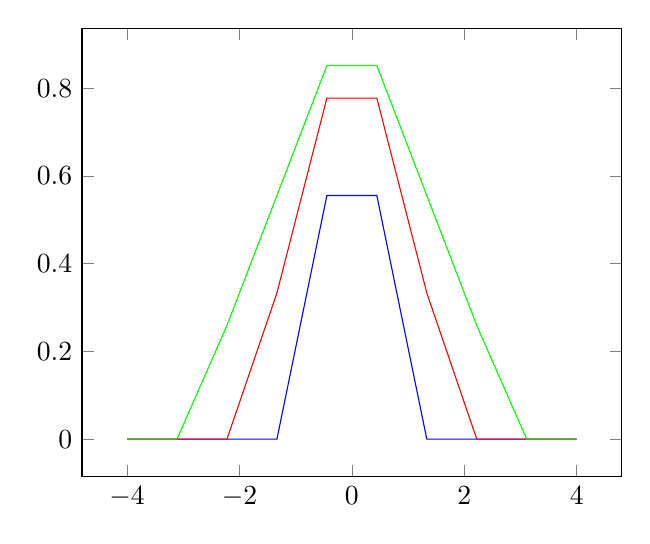
\begin{tikzpicture}
    \begin{axis}
    \addplot[domain=-4:4, samples=10, color=blue,]{max(x-1,0) + max(x+1,0) - 2*max(x,0)};
    \addplot[domain=-4:4, samples=10, color=red,]{max(x/2-1,0) + max(x/2+1,0) - 2*max(x/2,0)};
    \addplot[domain=-4:4, samples=10, color=green,]{max(x/3-1,0) + max(x/3+1,0) - 2*max(x/3,0)};
    \end{axis}
\end{tikzpicture}
    \caption{Illustration of the so-called ``bump'' function $\psi_a(x)$ used in the proof of \cref{lem:encoding-indicator-func2} with different exemplary values for $a$.}
    \label{fig:bump_function}
\end{figure}

We can now leverage all our lemmas to prove the overall theorem that any function $\cA$ computable by a \gnn can also be computed by \wlnn.
\begin{proof}[Proof of \cref{theorem:gnn_in_1wl}]\label{prof:gnn_in_1wl}
    Let $\cA$ be a function that works over $\cX$ to $\Rb$ computed by a \gnn model. We will prove that $\cA$ is \wlnn computable by decomposing the function and then argue that the decomposition is computable by a \wlnn model. For this let $G \in \cX$ be an arbitrary input graph, we can decompose $\cA(G)$ as follows:
    \begin{align}
        \cA(G) &= \Bigl( \ \frac{1}{|\cX/\!{\wliso}(G)|}\sum_{G^* \in \cX} \mathds{1}_{G \wliso G^*} \Bigr) \cdot \cA(G) \label{eq:gnn_decomposition1}\\
        &= \sum_{G^* \in \cX} \frac{1}{|\cX/\!{\wliso}(G)|} \cdot \cA(G) \cdot \mathds{1}_{G \wliso G^*} \label{eq:gnn_decomposition2}\\
        &= \sum_{G^* \in \cX} \frac{1}{|\cX/\!{\wliso}(G^*)|} \cdot \cA(G^*) \cdot \mathds{1}_{G \wliso G^*} \label{eq:gnn_decomposition3}\\
        &= \sum_{G^* \in \cX} \frac{\cA(G^*)}{|\cX/\!{\wliso}(G^*)|}  \cdot \varphi_{G^*}(G) \label{eq:gnn_decomposition4}
    \end{align}
    where $\cX/\!{\wliso}(G)$ denotes the set of all graphs that are equivalent to $G$ according to the $\wliso$ relation. We explain each equation step by step:
    \begin{itemize}[leftmargin=9em]
        \item[\cref*{eq:gnn_decomposition1}:] Multiplying $\cA(G)$ by the factor in the parentheses is correct because it is equal to $1$. This is because the sum ``counts'' the number of graphs $G^* \in \cX$ that are indistinguishable from the input graph $G$ by the \wl isomorphism test, and then the count is divided by the number of graphs in the equivalence class of $G$, which is the same as the count.
        \item[\cref*{eq:gnn_decomposition2}:] We can move both the factor $\cA(G)$ and $\frac{1}{|\cX/\!{\wliso}(G)|}$ into the sum by using the distributive property of the space $\Rb$.     
        \item[\cref*{eq:gnn_decomposition3}:] Due to the output of the indicator function $\mathds{1}$ being either $0$ or $1$, we can infer that the inner product of each summand can only be nonzero if $G^*$ is indistinguishable by the \wl isomorphism test from $G$. This implies that both are in the same equivalence class in these cases, such that $|\cX/\!{\wliso}(G)|$ is equal to $|\cX/\!{\wliso}(G^*)|$.\\
        Additionally, since \gnns are, at most, as good as the \wl algorithm in distinguishing pairs of non-isomorphic graphs (\cite{Morris2018,Xu2018}), we can use the fact that for every graph $G^* \in \cX$: if $G^* \wliso G$, then $\cA(G^*) = \cA(G)$. Using the same reasoning with the indicator function, we can replace the term $\cA(G)$ by $\cA(G^*)$.
        \item[\cref*{eq:gnn_decomposition4}:] Utilizing \cref{lem:encoding-indicator-func2}, we can replace the indicator function with $\varphi_{G^*}(G)$.
    \end{itemize}
    In conclusion, we have decomposed the \gnn function $\cA(G)$ such that the only factors that depend on the input graph $G$ are the functions $\varphi_{G^*}$, which take $G$ as input. This observation implies that all other factors are constants. Consequently, we can reason that the entire decomposition can be computed by a multilayer perceptron with a single layer, which takes the output of all $\varphi_{G^*}$ for all $G^* \in \cX$, applied to the input graph $G$. The multilayer perceptron then multiplies each of these values with the constant $\frac{\cA(G^*)}{|\cX/\!{\wliso}(G^*)|}$ and takes the sum. The existence of such a multilayer perceptron is evident, and when combined with \cref{lem:composition_lemma}, we can assert that this composition is \wlnn computable.

    Important to note, we can only do this since $\cX$ is finite, making the overall sum finite and the cardinality of $\cX/\!{\wliso}(G^*)$ well-defined for all graphs.
\end{proof}

\subsection{Proof of \cref*{theorem:1wl_in_gnn}: ``$\wlnn \subseteq \gnn$''}
In this section, we will prove the converse direction. Similar to the previous subsection, we will begin by introducing a set of lemmas that will play a crucial role in proving \cref{theorem:1wl_in_gnn}.

We start by showing the existence of a collection of functions computable by \gnns that is \wldisc. For the proof, we will devise message-passing layers for a \gnn that effectively compute a single iteration of the \wl algorithm per layer. Afterward, we show that with a proper choice of the \textsf{Readout} function, we construct a collection of \gnn functions that is \wldisc. 
Although prior works by \cite{Morris2018} and \cite{Xu2018} have already demonstrated how to construct message-passing layers to compute a single iteration of the \wl algorithm per layer, we include our own construction with our notation in the proof for two crucial reasons. Firstly, it ensures the completeness of our proof without assuming major parts. Secondly, and most importantly, it effectively highlights the remarkable similarities and key distinctions between the \wl algorithm and \gnns in general.
\begin{lemma}[GNN \wldisc]\label{lem:gnn_1wl_disc}
    There exists a collection $\cC$ of functions from $\cX$ to $\Rb$ computable by \gnns that is \wldisc.
\end{lemma}

\begin{proof}
    Due to $\cX$ being finite, we define the constants $n, m, k$ as follows:
    \begin{equation*}
        n := \max_{G \in \cX} |V(G)|, \quad  m := \sum_{G \in \cX} |V(G)|, \quad\text{and}\quad k := 1 + \max_{\substack{G \in \cX \\ v \in V(G)}} |l_G(v)|,
    \end{equation*}
    such that $n$ is the maximum number of nodes of any graph in $\cX$, $m$ is the total number of nodes of the set $\cX$, and $k$ is the largest label of any node of a graph in $\cX$ plus $1$.

    We will utilize these constants to construct the collection of functions $\cC := \{ \cA_c \mid c \in \Nb \}$ that is \wldisc. For the remainder of this proof, we first describe the construction of an arbitrary $\cA_c \in \cC$ and afterward, prove that the collection $\cC$ is \wldisc.

    Each $\cA_c$ consists of $n$ message-passing layers. We define the input layer $f^{(0)}(v) \coloneqq v$ as the identity functions such that there is no preprocessing of the node labels. Further, we define every other layer $t$ with $1 \leq t \leq n$ as follows:
    \begin{align*}
        f^{(t)}(v) \coloneqq f^{(t)}_{\text{merge}}(f^{(t-1)}(v), \ \MSopen f^{(t-1)}(u) \mid u \in \cN(v)\MSclose).
    \end{align*}
    Here $f^{(t)}_{\text{merge}}$ is an injective function that maps its input into its codomain:
    \begin{equation*}
       \{ i \in \Nb \mid k + (t-1) \cdot m \ \leq \  i \ \leq \ k + t \cdot m \}
    \end{equation*}
    This function exists due to the finiteness of $\cX$. We can upper bound the cardinality of its domain, the number of unique tuples, by the total number of nodes in $\cX$, which is $m$, and since the cardinality of its codomain is exactly $m$, we can conclude the existence of the function.

    Next, we will define the \textsf{Readout} function of $\cA_c$ to be the function that returns the number of nodes colored as $c$ in the coloring of $f^{(n)}$.
    
    By leveraging the results of \textit{theorem 3} from the work of \cite{Xu2018}, we can infer that each layer of each $\cA_c$ computes a single iteration of the \wl algorithm. This observation makes sense as the update equation for each layer injectively maps each tuple to a previously unused color, similar to how the \textsf{Relabel} function of the \wl algorithm works. Moreover, since the \wl algorithm terminates on any graph $G \in \cX$ after at most $|V(G)| \leq n$ iterations, the coloring computed by the layers of each $\cA_c$ effectively performs $n$ iterations of the \wl algorithm when applied to any graph $G \in \cX$. Due to the convergence behavior of the \wl algorithm, these additional iterations do not increase the expressiveness of the colorings computed by each $\cA_c$, such we can conclude for any graph $G \in \cX$:
    \begin{equation*}
       \forall c \in \Nb: |\{ v \in V(G) \mid  f^{(n)}(v) = c \}| = |\{ v \in V(G) \mid  \wl(G)(v) = c \}|,
    \end{equation*}
    which states that the colorings are equal for a bijection $\phi : \Nb \rightarrow \Nb$, such that we can infer that they are equally expressive for distinguishing non-isomorphism.

    To prove that the collection $\cC$ is \wldisc, we need to show two properties: 1) Each function in the collection is permutation invariant, and 2) For each pair of graphs in $\cX$ distinguishable by the \wl isomorphism test, there must exist a function in the collection that also distinguishes the pair.
   
    For the first property, by \cref{def:gnn} of \gnns, all functions computed by \gnns are permutation-invariant.
    Regarding the second property, consider $G_1, G_2 \in \cX$ with $G_1 \not\wliso G_2$. Let $C_1$ and $C_2$ represent the final colorings computed by the $\wl$ algorithm when applied to $G_1$ and $G_2$, respectively. Since $G_1 \not\wliso G_2$, there exists a color $c \in \Nb$ such that $\hist_{G_1,C_1}(c) \neq \hist_{G_2,C_2}(c)$. Since, we know that each $\cA_c$ computes equally expressive colorings of $G_1$ and $G_2$, we know that there exists a $c' \in \Nb$, such that $\cA_{c'}(G_1) \neq \cA_{c'}(G_2)$.
\end{proof}
 
Similar to the proof in the previous subsection, we will use \cref{lem:composition_lemma_gnn} to introduce the ability to construct \gnns that take in as input multiple \gnns and then apply a multilayer perceptron to the combined output. This insight is leveraged in the following two corollaries in the proof, as well as in the final proof.

\begin{lemma}[\gnn Composition]\label{lem:composition_lemma_gnn}
    Let $\cC$ be a collection of functions computable by \gnns. Further, let  $\cA_1, \dots , \cA_n \in \cC$ and $\mlp^\bullet$ a suitable multilayer perceptron, then the function $\hat{\cA}(\cdot) \coloneqq \mlp(\cA_1(\cdot), \dots, \cA_n(\cdot))$ is also computable by a \gnn.
\end{lemma}

\begin{proof}
    Before we begin the proof, we briefly introduce two notations. For any $x \in \Rb^d$, we will use the notation $x[i]$ to indicate the $i$.th element of the vector $x$. Additionally, we indicate the merge and aggregation function used in layer $t$ by $\cA_i$ as $f^{(t)}_{\text{merge}, i}$ and $f^{(t)}_{\text{agg}, i}$. Similarly, we denote the \textsf{Readout} function as $\textsf{Readout}_i$ and the input function of $\cA_i$ as $f^{(0)}_i$.
    
    We will prove the lemma by giving a construction of a \gnn model computing $\hat{\cA}$. For the ease of readability and to reduce the complexity of the subsequent construction, we assume that for all $\cA_i$ its functions $f^{(t)}_{\text{merge}, i}, f^{(t)}_{\text{agg}, i}$ and $\textsf{Readout}_i$ map into the one-dimensional space $\Rb$ for all layers $t$. With this assumption, we avoid the need for a formal notation of the number of dimensions each of these functions map to.

    Let $T$ be the maximum number of layers of all $\cA_1, \dots, \cA_n$. We construct the \gnn $\hat{\cA}$ with $T$ layers, with the input layer working as follows on an input graph $G$:
    \begin{align*}
        \forall v \in V(G): \ \hat{f}^{(0)}(v) \coloneqq \begin{bmatrix}
            f^{(0)}_1(v)\\
            \vdots\\
            f^{(0)}_n(v)
        \end{bmatrix},
    \end{align*}
    and each other layer $0 < t \leq T$ utilizing the merge $\hat{f}^{(t)}_{\text{merge}}$ and aggregation $\hat{f}^{(t)}_{\text{agg}}$ functions as constructed in the following:
    \begin{align*}
        \hat{f}^{(t)}_{\text{merge}} (\hat{f}^{(t-1)}(v), \ Agg) &:= \begin{bmatrix}
            f^{(t)}_{\text{merge}, 1}(\hat{f}^{(t-1)}(v)[1],\ Agg[1])\\
            \vdots\\
            f^{(t)}_{\text{merge}, n}(\hat{f}^{(t-1)}(v)[n],\ Agg[n])
        \end{bmatrix},\quad \text{and}\\
        \hat{f}^{(t)}_{\text{agg}}(\MSopen \hat{f}^{(t-1)}(w) \mid w \in \mathcal{N}(v) \MSclose ) &:= \begin{bmatrix}
            f^{(t)}_{\text{agg}, 1}(\MSopen \hat{f}^{(t-1)}(w)[1] \mid w \in \mathcal{N}(v) \MSclose)\\
            \vdots\\
            f^{(t)}_{\text{agg}, n}(\MSopen \hat{f}^{(t-1)}(w)[n] \mid w \in \mathcal{N}(v) \MSclose)
        \end{bmatrix}.
    \end{align*}
    Note that, not all $\cA_i$ will be comprised of $T$ layers, such that for these cases the functions $f^{(t)}_{\text{merge}, i}$ and $f^{(t)}_{\text{agg}, i}$ will not be defined for all $t \in [T]$. In these cases, we define the functions as follows:
    \begin{align*}
        f^{(t)}_{\text{merge}, i}(\hat{f}^{(t-1)}(v), \ Agg) &\coloneqq \hat{f}^{(t-1)}(v), \quad \text{and}\\
        f^{(t)}_{\text{agg}, i}(\MSopen \hat{f}^{(t-1)}(w) \mid w \in \mathcal{N}(v) \MSclose) &\coloneqq 0.
    \end{align*}
    This definition of $f^{(t)}_{\text{merge}, i}$ and $f^{(t)}_{\text{agg}, i}$ results in the fact that the representation computed in the last layer of $\cA_i$ is forwarded to the last layer $T$ of $\hat{\cA}$. Finally, we construct the \textsf{Readout} function of $\hat{\cA}$ as follows:
    \begin{align*}
        \textsf{Readout}(\MSopen \hat{f}^{(T)}(v) \mid v \in V(G) \MSclose) \coloneqq \mlp^\bullet \circ \begin{bmatrix}
            \textsf{Readout}_1(\MSopen \hat{f}^{(T)}(v)[1] \mid v \in V(G) \MSclose)\\
            \vdots\\
            \textsf{Readout}_n(\MSopen \hat{f}^{(T)}(v)[n] \mid v \in V(G) \MSclose)
        \end{bmatrix}.
    \end{align*}
    With this, the proof concludes. Note that this proof can easily be extended to work without the assumption of each function mapping into a one-dimensional space.
\end{proof}

As a consequence of the previous two lemmas, we find ourselves in a similar position as at the beginning of the proof in \cref{sec:proof_theorem:1wl_in_gnn}. Specifically, we have established, through \cref{lem:gnn_1wl_disc}, the existence of a collection $C$ of functions that can be computed by \gnns and can effectively distinguish any pair of graphs that are also distinguishable by the \wl algorithm. Furthermore, with \cref{lem:composition_lemma_gnn}, we have demonstrated that the composition of multiple \gnns and a multilayer perceptron remains computable by a single \gnn. Consequently, we can use the same proofs of \cref{lem:encoding-indicator-func1,lem:encoding-indicator-func2} to derive the \cref{lem:encoding-indicator-func1_gnn,lem:encoding-indicator-func2_gnn}. 

\begin{corollary}\label{lem:encoding-indicator-func1_gnn}
    Let $\cC$ be a collection of functions from $\cX$ to $\Rb$ computable by \gnns that is \wldisc. Then for all $G^* \in \cX$, there exists a function $h_{G^*}$ from $\cX$ to $\Rb$ computable by \gnn, such that on any input $G \in \cX: h_{G^*}(G) = 0$, if and only if, $G \wliso G^*$.
\end{corollary}
\begin{corollary}\label{lem:encoding-indicator-func2_gnn}
    Let $\cC$ be a collection of functions from $\cX$ to $\Rb$ computable by \gnns such that for all $G^* \in \cX$, there exists $h_{G^*} \in \cC$ satisfying $h_{G^*}(G) = 0 $, if and only if, $G \wliso G^*$, for all $G \in \cX$. Then for every $G^* \in \cX$, there exists a function $\varphi_{G^*} $ computable by \gnns such that for all $G \in \cX$: $\varphi_{G^*}(G) = \mathds{1}_{G \wliso G^*}$.
\end{corollary}

In conclusion, the corollaries establish the computability of the indicator function $\mathds{1}_{G_1 \wliso G_2}$ over the set $\cX$ by a \gnn. Building upon these results, we can now utilize all our lemmas to prove the theorem, which states that any function $\cB$ computable by a \wlnn can also be computed by a \gnn.

\begin{proof}[Proof of \cref*{theorem:1wl_in_gnn}]
    Let $\cB$ be a function that works over $\cX$ to $\Rb$ computed by a \wlnn model. We will prove that $\cB$ is \gnn computable by decomposing the function and then argue that the decomposition is computable by a \gnn model. For this let $G \in \cX$ be an arbitrary input graph, we can decompose $\cB(G)$ as follows:
    \begin{align}
        \cB(G) &= \Bigl( \ \frac{1}{|\cX/\!{\wliso}(G)|}\sum_{G^* \in \cX} \mathds{1}_{G \wliso G^*} \Bigr) \cdot \cB(G) \nonumber\\
        &= \sum_{G^* \in \cX} \frac{1}{|\cX/\!{\wliso}(G)|} \cdot \cB(G) \cdot \mathds{1}_{G \wliso G^*} \nonumber\\
        &= \sum_{G^* \in \cX} \frac{1}{|\cX/\!{\wliso}(G^*)|} \cdot \cB(G^*) \cdot \mathds{1}_{G \wliso G^*} \label{eq:wlnn_decomposition3}\\
        &= \sum_{G^* \in \cX} \frac{\cB(G^*)}{|\cX/\!{\wliso}(G^*)|}  \cdot \varphi_{G^*}(G) \label{eq:wlnn_decomposition4}
    \end{align}
    where $\cX/\!{\wliso}(G)$ denotes the set of all graphs that are equivalent to $G$ according to the $\wliso$ relation. Since the decomposition is very similar to the one present in the proof of \cref{theorem:gnn_in_1wl}, we will only provide reasoning for the correctness of \cref{eq:wlnn_decomposition3,eq:wlnn_decomposition4}. For all other equations, refer to the explanation provided in the proof of \cref{theorem:gnn_in_1wl}
    \begin{itemize}[leftmargin=9em]
        \item[\cref*{eq:wlnn_decomposition3}:] Due to the output of the indicator function $\mathds{1}$ being either $0$ or $1$, we can infer that the inner product of each summand can only be nonzero if $G^*$ is indistinguishable by the \wl isomorphism test from $G$. Using \cref{lem:wl_relation_equivalence}, we know that for every graph $G^* \in \cX$: if $G^* \wliso G$, then $\cB(G^*) = \cB(G)$.
        \item[\cref*{eq:wlnn_decomposition4}:] Utilizing \cref{lem:encoding-indicator-func2_gnn}, we can replace the indicator function with $\varphi_{G^*}(G)$.
    \end{itemize}
    In conclusion, we have decomposed the \gnn function $\cB(G)$ such that the only factors that depend on the input graph $G$ are the functions $\varphi_{G^*}$, which take $G$ as input. This observation implies that all other factors are constants. Consequently, we can reason that the entire decomposition can be computed by a multilayer perceptron with a single layer, which takes the output of all $\varphi_{G^*}$ for all $G^* \in \cX$, applied to the input graph $G$. The multilayer perceptron then multiplies each of these values with the constant $\frac{\cB(G^*)}{|\cX/\!{\wliso}(G^*)|}$ and takes the sum. The existence of such a multilayer perceptron is evident, and when combined with \cref{lem:composition_lemma}, we can assert that this composition is \wlnn computable.

    Important to note, we can only do this since $\cX$ is finite, making the overall sum finite and the cardinality of $\cX/\!{\wliso}(G^*)$ well-defined for all graphs.
\end{proof}